
\section{Knowledge and reasoning distillation} \label{sec:distillation}

\begin{figure}[htb]
  \centering
  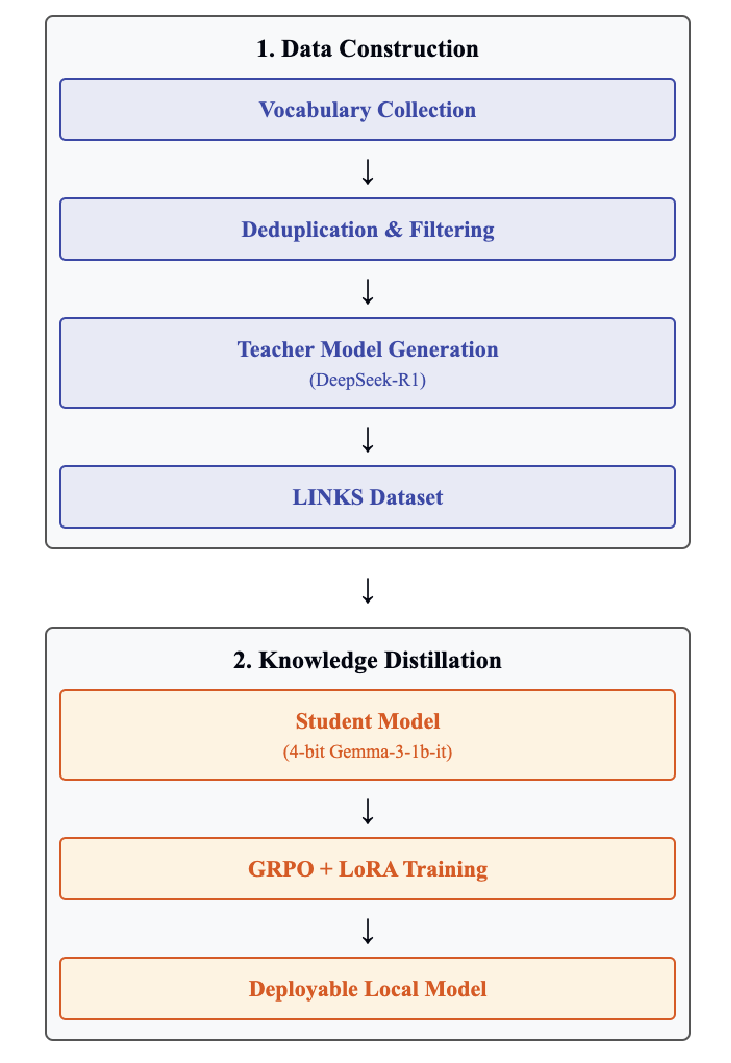
\includegraphics[width=\linewidth]{figures/pipeline.pdf}
  \caption{\linksys pipeline. The pipeline consists of two main components: (1) CoT data generation and (2) model distillation. We generate a dataset of mnemonics with reasoning traces using a large language model (LLM) as a teacher. Then we distill the reasoning capabilities of the teacher model into a smaller student model using GRPO \Cref{app:grpo}. Finally, we obtain \linksys, a smaller model that can generate mnemonics through linguistic reasoning.}
  \label{fig:distillation}
\end{figure}

\subsection{Preparation} \label{sec:data-prep}
We first created a comprehensive training dataset. Following best practices in synthetic data generation with LLMs \citetext{\citealp{longLLMsDrivenSyntheticData2024b}, \citealp{openthoughtsteamOpenThoughts2025}}, we designed a data construction pipeline with key components (\Cref{fig:distillation}).

\paragraph*{Vocabulary selection} \label{sec:vocab-selection}
We collected 5,000 distinct words from three main sources: English as a foreign language tests (TOEFL iBT, IELTS Academic), standardized tests with verbal reasoning (SAT, GRE), and CEFR C1/C2 word lists. This ensured coverage of academic and abstract vocabulary that would benefit from mnemonic devices. After fuzzy-matching deduplication (threshold 95\%), we refined the dataset and performed stratified random sampling (stratified by linguistic features used) to obtain 2,000 distinct vocabulary for post-training.

\paragraph*{Prompt design and model selection} Based on \cref{sec:icl-performance}'s findings, we designed system and user prompts, focusing on the 10-shot CoT approach that demonstrated superior performance in eliciting linguistic reasoning and creating memorable, \lgms.

\subsection{Dataset generation} \label{sec:data-gen}

Using our optimized prompts and vocabulary list, we generated the \links dataset of approximately 2,000 entries, each containing:

\begin{equation}
(\tau_i, m_i, e_i) \in \mathcal{D}
\end{equation}

where $\tau_i$ represents the reasoning trace exploring linguistic features, $m_i$ the generated mnemonic, and $e_i$ an example sentence for vocabulary $i$. The dataset creation process can be formalized as:

\begin{equation}
(\tau_i, m_i, e_i) = f_{\text{teacher}}(v_i; p_{\text{CoT}})
\end{equation}

where $f_{\text{teacher}}$ is the teacher model function, $v_i$ is vocabulary $i$, and $p_{\text{CoT}}$ is our 10-shot CoT prompt.

\subsection{Quality control} To ensure the quality of the generated mnemonics, we implemented a multi-step validation process. We first filtered out any entries that did not meet our structured output format or contained incomplete reasoning traces. We then performed a manual review of a random sample of 200 entries to assess the linguistic grounding and coherence of the mnemonics. This review process involved checking for clear connections between the vocabulary and the mnemonic, as well as ensuring that the example sentence accurately reflected the vocabulary's meaning.

\subsection{Training and inference} \label{sec:training-inference}
To transfer the linguistic reasoning capability to a smaller model, we implemented a distillation process using Group Relative Policy Optimization (GRPO).

We selected Google's \studentmodel \citep{gemma-teamGemma3Technical2025} as our student model due to its balance of performance and size (1 billion parameters). It can handle general-purpose tasks in multiple languages, and demonstrate instruction-following abilities. We used a 4-bit quantized version to further reduce memory requirements while maintaining performance \citep{dettmersQLoRAEfficientFinetuning2023}.

\paragraph*{Group Relative Policy Optimization (GRPO)} We employed GRPO \citep{DeepSeek-AIDEEPSEEKR12025} to distill the reasoning capabilities into the student model. For each input prompt $q$ generating a vocabulary $v$, the model produces $G$ candidate outputs:

\begin{equation}
O_q = \{o_1, o_2, \ldots, o_G\}
\end{equation}

These outputs are evaluated using reward functions $r_j$ that output scores, with the overall reward for output $i$ calculated as:

\begin{equation}
r_i = \sum_{j=1}^{J} w_j r_j(o_i, v)
\end{equation}

where $w_j$ is the weight for reward function $j$. We provide more technical details in \Cref{app:grpo}, including the policy loss to be minimized.

We defined three reward functions $r$ that encode essential characteristics of effective mnemonics:
\numlist{1} adherence to the structured format with reasoning, mnemonic, and example,
\numlist{2} usage of the target vocabulary in the mnemonic, penalizing bad mnemonics such as acronyms, and
\numlist{3} explicit incorporation of linguistic features in \Cref{tab:linguistic-features} or a reasonable custom feature.

We assigned higher weights to criterion 3, and generated $G=2$ candidates per training example to enable learning from comparisons. Training was performed on a single NVIDIA H100 GPU for approximately 4 hours (more details in \Cref{app:grpo-config}).

\paragraph*{Low-Rank Adaptation (LoRA)} We trained \studentmodel using GRPO wrapped in LoRA layers (\Cref{app:lora-config}) to reduce the number of trainable parameters and rank-stabilized LoRA that maintains stability for adapters with higher ranks.
